\chapter{Évaluation à large couverture}\label{chap:large-scale-eval}

% on veut aller plus loin dans ce chapitre
% on quitte le domaine journalistique pour aller voir les autres domaines
% on étend aussi en terme de méthodes

Dans le chapitre~\ref{chap:kptimes}, nous avons introduit et évalué KPTimes, le jeu de données que nous avons construit.
Nous l'avons comparé à d'autres jeux de données rassemblant les mêmes genres de documents et nous nous en sommes servi pour évaluer les performances de méthodes de production automatique de mots-clés.
%
Nous avons aussi présenté dans les chapitre~\ref{chap:concepts} et \ref{chap:kw_production} les principales méthodes de production automatique de mots-clés proposées par la communauté scientifique.
Pour mesurer les progrès réalisés par ces différentes méthodes et ainsi orienter les travaux de recherches il est nécessaire de comparer ces méthodes.
Malheureusement, elles sont difficilement comparables.
En effet, si nous examinons, par exemple, les articles de \citet{meng_deep_2017}, \citet{florescu_positionrank:_2017} et \citet{teneva_salience_2017}, tous publiés en 2017 à la conférence ACL, nous remarquons que ni les jeux de données, ni les paramètres, ni les protocoles d'évaluation ne sont comparables. Il est donc impossible de savoir quelle méthode est la plus performante.
Il en va de même pour les méthodes en chaîne de traitement.
Même si les jeux de données et métriques utilisées semblent se standardiser, le processus d'évaluation ainsi que les pré-traitements ne sont pas normalisés.
La mise en \oe{}uvre de ces étapes peut donc impacter les performances rapportées.

C'est pourquoi, dans ce chapitre, nous conduisons une évaluation de grande envergure sur des jeux de données variant tant sur le genre de documents que sur la taille et le type d'annotation. Nous comparons également un grand nombre de méthodes qui représentent les différentes catégories des méthodes proposées par la communauté scientifique: statistiques, fondées sur les graphes et neuronales. %FirstPhrases, TextRank, Tf$\times$Idf, PositionRank, MPRank, EmbedRank, Kea, CopyRNN, CorrRNN.
%En effet, il est difficile d'avoir un aperçu des performances des méthodes proposées
%
Pour cette évaluation, nous adoptons un cadre expérimental strict avec une chaîne de pré-traitements, une sélection des candidats et un protocole d'évaluation partagé.
Ce cadre expérimental va nous permettre de répondre aux questions suivantes: 

\begin{enumerate}
    \item Quels progrès ont été réalisés en matière de production de mots-clés depuis les premières méthodes statistiques?
    \item Quel est l'impact de l'utilisation de mots-clés de référence non experts pour l'entraînement et l'évaluation des méthodes de production automatique de mots-clés ?
    \item Quelles méthodes et quels jeux de données devraient être utilisés pour mieux comprendre les avantages et les inconvénients des nouvelles méthodes ?
\end{enumerate}


\section{Cadre expérimental}

%Outre la variation dans le choix des jeux de données et des méthodes de base, il existe également des différences importantes dans les paramètres et les mesures d'évaluation entre les études précédentes.
%
%Pour pallier à ce manque de comparabilité, nous utilisons les mêmes outils de prétraitement, les mêmes paramètres et la même procédure d'évaluation dans toutes nos expériences.
Dans cette section, nous détaillons successivement les jeux de données, les méthodes testées, les paramètres expérimentaux et les métriques utilisées dans cette évaluation.


\subsection{Jeux de données}
\label{sec:benchmark_datasets}

Nous utilisons 9 jeux de données qui sont représentatifs des différents genres de documents classiquement employés pour évaluer les méthodes de production automatique de mots-clés.
Ces jeux de données représentent aussi différents types d'annotation: auteurs, indexeurs, lecteurs et éditeurs.
Les statistiques détaillées des jeux de données sélectionnés sont présentées dans la section~\ref{sec:framework_datasets}.
Nous avons regroupé ces jeux de données en trois catégories en fonction du genre et de la taille des documents qu'ils contiennent:

\begin{itemize}
    %\item articles scientifiques: ACM~\cite{krapivin_large_2009}, SemEval-2010~\cite{kim_semeval-2010_2010}, PubMed~\cite{schutz_keyphrase_2008} ;
    %\item notices scientifiques: Inspec~\cite{hulth_improved_2003}, WWW~\cite{caragea_citation-enhanced_2014}, KP20k~\cite{meng_deep_2017} ;
    %\item articles journalistiques: DUC-2001~\cite{wan_single_2008}, KPCrowd~\cite{marujo_supervised_2012}, KPTimes~\cite{gallina_kptimes_2019}.
    
    \item articles scientifiques: ACM, SemEval-2010, PubMed;
    \item notices scientifiques: Inspec, WWW, KP20k;
    \item articles journalistiques: DUC-2001, KPCrowd, KPTimes.
\end{itemize}

Nous utilisons les documents tels qu'ils ont été distribués: nous ne cherchons pas à améliorer la qualité des données en procédant, par exemple, à un nettoyage plus poussé.
Les travaux de \citet{boudin_how_2016} montrent, en effet, qu'un nettoyage plus poussé améliore significativement les performances des méthodes.
Les jeux de données KP20k et PubMed, par exemple, contiennent des noms de molécules et des formules mathématiques.
Ces entités gagneraient à être segmentées en un seul mot et remplacées par un mot spécial.
En effet, une mauvaise segmentation de ces entités va fausser leur étiquetage morphosyntaxique ou permettre aux modèles d'en retourner des sous-chaînes qui n'ont pas de sens en dehors de leur contexte.


%et nous sommes conscients que les performances rapportés peuvent être augmentées en améliorant la qualité des prétraitements.

\subsection{Méthodes}

Dans cette section, nous listons les méthodes de base et état de l'art choisis pour notre évaluation.
Toutes ces méthodes ont été réimplémentées par nos soins. Les méthodes en chaîne de traitement, en particulier, le sont dans l'outil PKE~\cite{boudin_pke_2016}.
Toutes les méthodes sont décrites en détail dans les sections~\ref{sec:methode-en-chaine-de-traitement} et \ref{methodes-de-bout-en-bout}.
Nous rappelons donc succinctement leur fonctionnement et justifions leur choix ci-dessous.

\paragraph{Méthodes de base}
%Il est indispensable de disposer de méthodes de base solides pour pouvoir comparer les résultats des modèles proposés.
%Dans les études précédentes, diverses méthodes de base ont été utilisées, ce qui complique l'analyse et l'interprétation des résultats rapportés.
Nous avons choisi trois méthodes dites \say{de base}, chacune associée à une caractéristique couramment utilisée dans les méthodes d'extraction de mots-clés: la position, la centralité et la fréquence.
Ces méthodes de base sont non supervisées, ce qui permet leur utilisation et l'analyse de leurs performances sur tous les jeux de données. Ces trois méthodes sont:
\begin{itemize}
    \item \textbf{FirstPhrases} qui utilise la position des mots-clés comme seul indicateur de l'importance des mots. La position en est un signal fort car les textes sont généralement écrits de manière à ce que les idées les plus importantes soient exprimées en premier~\cite{marcu_rhetorical_1997}. FirstPhrases extrait, ainsi, les $N$ premiers mots-clés candidats d'un document.
    \item \textbf{TextRank}~\cite{mihalcea_textrank:_2004} est la première méthode fondée sur les graphes et elle est souvent utilisée comme base de comparaison à d'autres méthodes. Le document est tout d'abord représenté sous forme de graphe où les mots correspondent aux n\oe{}uds et les relations de cooccurrence aux arêtes. Ensuite, l'algorithme d'ordonnancement de n\oe{}uds PageRank est exécuté pour calculer la centralité de chaque mot dans le graphe.
    \item \textbf{\tfidf{}}~\cite{salton_term-weighting_1988} est utilisée dans de nombreuses études comparatives~\cite[\textit{inter alia}]{kim_semeval-2010_2010,meng_deep_2017}.
    Ce schéma de pondération mesure la spécificité et la fréquence de chaque mot dans un document par rapport à un corpus.
    Cette méthode, bien que simple, obtient dans certains cas des performances compétitives avec les modèles neuronaux de bout-en-bout.
\end{itemize}

\paragraph{Méthodes non supervisées}

Nous avons ensuite sélectionné trois méthodes non supervisées de l'état de l'art qui pallient certains manques des méthodes de base:
\begin{itemize}
    \item \textbf{PositionRank}~\cite{florescu_positionrank:_2017} est une méthode fondée sur les graphes qui incorpore la position et la fréquence des mots dans le calcul de leur centralité. Elle combine ainsi les trois caractéristiques utilisées par les méthodes de base.
    \item \textbf{MPRank}~\cite{boudin_unsupervised_2018} s'appuie sur un graphe multipartite pour regrouper les mots-clés candidats sur la base de leur similarité textuelle. Cela permet de produire des mots-clés moins redondants et de mutualiser l'information des mots-clés similaires.
    \item \textbf{EmbedRank}~\cite{bennani-smires_simple_2018} pondère les mots-clés candidats par leur similarité au document. Cette similarité est établie par la distance cosinus entre les représentations denses des mots-clés candidats et du document. Les représentations denses sont obtenues grâce à une technique de plongement de phrases~\cite{pagliardini_unsupervised_2018} qui capture la sémantique de ces entités.
    \end{itemize}

\paragraph{Méthodes supervisées}

Nous avons retenu trois méthodes supervisées état de l'art:
\begin{itemize}
    \item\textbf{Kea}~\cite{witten_kea:_1999} est l'une des premières méthodes supervisées de production de mots-clés.
    Elle utilise la position et le \tfidf{} des mots-clés candidats pour les classifier comme mot-clé ou non.
    Elle nous permet de mesurer l'écart de performance avec les méthodes neuronales récentes, bien plus complexes et gourmandes en données d'entraînement.
    \item\textbf{CopyRNN}~\cite{meng_deep_2017} est une méthode neuronale fondée sur le paradigme encodeur-décodeur avec mécanisme d'attention et de copie.
    Le mécanisme de copie permet au modèle de générer des mots peu fréquents qui ne font pas partie du vocabulaire de sortie mais apparaissent dans le document.
    Le mécanisme d'attention, quant à lui, permet au modèle de générer des mots-clés qui capturent un aspect spécifique en portant attention aux parties du document liées à cet aspect.
    Contrairement aux autres méthodes choisies, CopyRNN possède la capacité de produire des mots-clés absents du document grâce à son processus génératif.
    \item \textbf{CorrRNN}~\cite{chen_keyphrase_2018} étend le modèle CopyRNN dans le but de produire des mots-clés moins redondants.
    Pour cela, le modèle apprend à générer les mots-clés en fonction des précédents.
    Un mécanisme de revue permet au modèle de porter attention à ces mots-clés déjà générés et un mécanisme de couverture informe le modèle des parties du document auxquelles il a déjà porté attention.

\end{itemize}

Notons que seules les méthodes génératives de bout-en-bout ont la capacité de générer des mots-clés absents, ce qui leur confère un avantage sur les autres méthodes.

%Le deuxième modèle que nous étudions est \textbf{TopicCoRank}~\cite{bougouin_keyphrase_2016}, une approche supervisée à base de graphe pour l'extraction de mots-clés.


\subsection{Paramètres expérimentaux}

Nous présentons ici les paramètres expérimentaux choisis pour notre évaluation à large couverture.
Nous décrivons ainsi les pré-traitements que nous appliquons aux documents, la méthode de sélection des mots-clés candidats retenue et les paramètres des méthodes.

%prétraitement des textes
\paragraph{Pré-traitement} Nous pré-traitons tous les documents des jeux de données à l'aide de Stanford CoreNLP~\cite{manning_stanford_2014} pour la tokenisation, le découpage des phrases et l'étiquetage morphosyntaxique.

%sélection des candidats
\paragraph{Sélection des candidats} Cette étape est particulièrement importante pour les méthodes en chaîne de traitement. Nous devons adopter une sélection qui minimise le silence et le bruit.
%
Pour une comparaison équitable, nous utilisons la même heuristique de sélection des candidats pour chaque méthode. Nous utilisons les séquences de noms adjacents précédés d'un ou plusieurs adjectifs  décrits par l'expression régulière suivante: \texttt{A*N+}.
%
Nous suivons la recommandation de~\citet{wang_how_2014} en conservant seulement les séquences de moins de cinq mots.
%
Les candidats sont ensuite filtrés en éliminant ceux qui ont moins de 3 caractères (\say{km}, \say{$\mu$m}), qui contiennent des symboles non alphanumériques (\say{$\alpha$ phényl}, \say{vs.}) ou bien des mots vides (\say{théorie chimique de}, \say{analyse des flux médiatiques d' informations}).

% librairie
\paragraph{Paramètres}
Nous avons implémenté les méthodes neuronales avec PyTorch~\cite{paszke_pytorch_2019} grâce à la bibliothèque AllenNLP~\cite{gardner_allennlp_2018}.
%paramétrages des modèles neuronaux
Pour les méthodes CopyRNN et CorrRNN nous utilisons les paramètres recommandés par les auteurs originaux: GRU bidirectionnel, vocabulaire de \num{50 000} mots et pour l'inférence, grâce à l'algorithme de recherche en faisceau, nous générons 200 mots-clés de six mots maximum.

Les méthodes en chaîne de traitement sont implémentées dans la bibliothèque \texttt{pke}~\cite{boudin_pke_2016}, et nous utilisons là encore les paramètres recommandés par les auteurs originaux.
Pour EmbedRank, nous utilisons la méthode \texttt{sent2vec} avec le modèle pré-entraîné \texttt{wiki\_bigrams} pour calculer les représentations denses des mots-clés candidats et du document.
\todo{décrire plus précisément les paramètres genre pour chaque méthode....}


\paragraph{Entraînement}
Les méthodes requérant un entraînement sont: \tfidf{}, Kea, CopyRNN et CorrRNN.

Nous entraînons \tfidf{} et Kea sur les ensembles d'entraînement s'ils sont disponibles.
Si un jeu de donnée ne possède pas d'ensemble d'entraînement, nous utilisons une procédure de validation croisée d'un contre tous (\foreign{leave-one-out}) sur l'ensemble de test.
C'est-à-dire que la méthode est entraînée grâce à l'ensemble des documents moins un, et cela pour chaque document.

Les méthodes CopyRNN et CorrRNN nécessitent de grandes quantités de données annotées pour être entraînées.
Ainsi, nous ne pouvons le faire qu'avec KP20k et KPTimes.
Les mots-clés des jeux de données d'articles scientifiques et de notices scientifiques sont inférés par les modèles entraînés sur KP20k et ceux des jeux de données d'articles journalistiques le sont par les modèles entraînés sur KPTimes.
%
Nous avons montré dans la section~\ref{sec:framework_datasets_discussion} qu'un nombre non négligeable de documents, apparaissant dans des ensembles de test, apparaissent aussi dans l'ensemble d'entraînement de KP20k.
L'entraînement d'un modèle avec ce jeu de données fausserait la comparaison des performances entre les différents jeux de données, certains seraient avantagés par rapport aux autres.
En particulier, \npercent{84} des documents de l'ensemble de test d'ACM apparaissent dans l'ensemble d'entraînement de KP20k.
Pour éviter ces problèmes, nous supprimons de l'ensemble d'entraînement de KP20k les documents communs aux ensembles de test et à cet ensemble d'entraînement.


\subsection{Métriques d'évaluation}

Bien qu'il n'y ait pas de consensus quant à la métrique la plus pertinente pour évaluer la qualité des mots-clés produits automatiquement, la stratégie d'évaluation la plus répandue consiste à rapporter la F@10 ou la F@5 (voir section~\ref{sub:framework_metrics}).
Nous choisissons donc de rapporter la F@10 car le nombre moyen de mots-clés dans les documents des jeux de données comparés est de 11,6.
Nous rapportons également une seconde métrique, la \map{}, pour évaluer l'ordonnancement des mots-clés ainsi que le test de Student apparié au niveau de 0,05 pour identifier les méthodes dont les performances sont significativement supérieures à celles des méthodes de base.

%ACM, SemEval,Pubmed(5.3+14.7+5.4)/3
%Inspec,WWW,KP20K(9.8+4.8+5.3)/3
%Duc,KPCRowd,KPTimes(8.1+46.2+5.2)/3
%
Nous observons que les méthodes de bout-en-bout sont évaluées séparément sur les mots-clés présents et les mots-clés absents, alors que les méthodes en chaîne de traitement sont évaluées sur l'intégralité de la référence.
Nous choisissons ici d'évaluer les méthodes sur l'ensemble de la référence.
% En effet, les méthodes récentes, en plus de la production de mots-clé à partir du contenu du document, sont capables de générer des mots-clé absents.
%
%Pour évaluer les performances globales d'ordonnancement des modèles, nous indiquons également les scores de \foreign{mean Average Precision} (mAP) des listes de mots-clé.
%
%Pour augmenter les correspondances nous utilisons l'implémentation de \texttt{nltk} du raciniseur de Porter\footnote{\url{https://www.nltk.org/api/nltk.stem.html\#nltk.stem.porter.PorterStemmer}}.


\subsection{Reproductibilité des résultats}

Malgré l'objectif de reproduire au plus près les résultats des articles originaux, des différences peuvent apparaître lors de la réimplémentation des méthodes.
Ces différences peuvent être liées à plusieurs facteurs tels que: des paramètres peu détaillés dans les articles originaux, des différences dans les pré-traitements ou le processus d'évaluation.
Ainsi, pour mesurer ces différences, nous comparons dans le tableau~\ref{tab:replicability} les performances obtenues par les méthodes que nous avons réimplémentées à celles rapportées dans les articles originaux.
%
Nous observons ainsi quelques différences, les plus importantes concernant les méthodes neuronales CopyRNN ($+2$) et CorrRNN (\num{-3.1}).
Mais nous considérons que ces différences ne sont pas assez significatives pour impacter la validité des conclusions de notre étude.

\input{5_comparaison_modeles/tables/replicability}

Pour CorrRNN cette différence de performance peut être liée à deux facteurs.
Le premier concerne les différences d'entraînement: l'article original de CorrRNN ajoute une partie des jeux de données SemEval-2010 et ACM à l'ensemble d'entraînement de KP20k, étape que nous n'avons pas suivie pour notre réimplémentation.
Le deuxième facteur est lié à l'évaluation.
En effet, dans l'article original, la méthode CorrRNN n'est pas évaluée sur KP20k, mais sur les jeux de données d'articles scientifiques NUS, SemEval-2010 et ACM.
Notre modèle réimplémenté étant entraîné sur des notices scientifiques (176 mots en moyenne) et notre GPU ne pouvant traiter l'entièreté de ces documents (9\,200 mots en moyenne), nous choisissons de nous comparer sur les documents d'ACM car il est possible d'en extraire le résumé (voir section~\ref{sec:framework_datasets}).
Ensuite, dans l'article original seuls les 400 premiers documents triés par ordre alphabétique d'ACM sont utilisés pour l'évaluation.
Pour mesurer l'impact de ce choix, nous évaluons notre modèle: sur l'\emph{ensemble} du jeu de données et obtenons 23,5 de F@10; sur les 400 premiers documents triés par \emph{ordre alphabétique} et obtenons 24,7 de F@10; sur les 400 premiers documents triés par \emph{ordre numérique} car les identifiants sont des nombres et obtenons 29,3 de F@10.
Ainsi en modifiant simplement la méthode de tri des documents nous obtenons un écart de 4,6 points de F@10.
Il est donc possible que la différence que nous obtenons provienne en partie de l'évaluation.

%Malgré une initialisation des poids entre \num{-1} et 1 telle que préconisée par \citet{meng_deep_2017,chen_keyphrase_2018}, nous remarquons que l'initialisation aléatoire influe significativement sur les performances en positif ou en négatif. Nous aurions pu tenter de réduire ces différences en moyennant les performances de plusieurs initialisations aléatoires.
Pour CopyRNN, les performances plus élevées de notre modèle peuvent être liées à un paramètre qui n'est pas décrit dans l'article mais apparaît dans le code partagé sur GitHub: la taille maximale des documents.
En effet, lors de l'entraînement les documents sont tronqués à 256 mots mais nous n'avons pas effectué cette étape lors de notre réimplémentation.
Ainsi, le modèle, ayant accès à plus d'informations, générerait de meilleurs mots-clés.

De plus, les poids des méthodes neuronales sont initialisés aléatoirement et introduisent donc une variabilité dans les performances obtenues. Pour minimiser cette variabilité nous aurions pu entraîner plusieurs fois le même modèle et moyenner les résultats de ces différents entraînement.

%D'autres paramètres, peu détaillés dans les  Des différences d'implémentations peuvent aussi jouer sur les performances, par exemple la transition entre l'état caché de l'encodeur et du décodeur n'est pas précisé dans les descriptions de CopyRNN et CorrRNN; il est possible de les concaténer, de les additionner ou d'appliquer une transformation non linéaire.

Pour la méthode Kea, les performances varient radicalement en fonction des implémentations: sur SemEval-2010, \citet{meng_deep_2017} rapporte une F@10 de 2,6 tandis que \citet{boudin_pke_2016} rapporte un score de 19,3.
L'implémentation que nous utilisons, basée sur celle de PKE, donne dans cette étude une F@10 de 19,5.
Cette grande variation de performance est également visible pour les méthodes de base en général, comme \tfidf{} ou TextRank, dont les paramètres sont peu décrits dans les articles qui les utilisent.
En effet, ces méthodes ne sont pas au c\oe{}ur du travail et ne sont évaluées qu'à titre de comparaison.



% a développer, pourquoi CopyRNN est à +2, pourquoi CorrRNN est à -4.3 ?
% en général: initialisation aléatoire, filtrage des documents d'entraînement de KP20k, tout les paramètres ne sont pas détaillés
% copyRNN: manque de détails, autre librairie
% corrRNN: manque de détails

\section{Résultats de l'évaluation}
\label{sec:large_eval_results}

\begin{sidewaystable}
%\begin{table}[ht!]
    \centering
    %\rotatebox{90}{%
    \resizebox{\linewidth}{!}{
    \begin{tabular}{r c@{\hspace*{2mm}}c c@{\hspace*{2mm}}c c@{\hspace*{2mm}}c | c@{\hspace*{2mm}}c c@{\hspace*{2mm}}c c@{\hspace*{2mm}}c | c@{\hspace*{2mm}}c c@{\hspace*{2mm}}c c@{\hspace*{2mm}}c}
    
        ~ &
        \multicolumn{6}{c}{\textit{Articles scientifiques}} &
        \multicolumn{6}{c}{\textit{Notices scientifiques}} &
        \multicolumn{6}{c}{\textit{Articles journalistiques}}
        \\
        
        \cmidrule(lr){2-7} \cmidrule(lr){8-13} \cmidrule(lr){14-19}
    
        ~ &
        \multicolumn{2}{c}{\textbf{PubMed}} &
        \multicolumn{2}{c}{\textbf{ACM}} &
        \multicolumn{2}{c}{\textbf{SemEval}} &
        \multicolumn{2}{c}{\textbf{Inspec}} &
        \multicolumn{2}{c}{\textbf{WWW}} &
        \multicolumn{2}{c}{\textbf{KP20k}} &
        \multicolumn{2}{c}{\textbf{DUC-2001}} &
        \multicolumn{2}{c}{\textbf{KPCrowd}} &
        \multicolumn{2}{c}{\textbf{KPTimes}} \\ 
        
        
        \cmidrule(lr){2-3} \cmidrule(lr){4-5} \cmidrule(lr){6-7}
        \cmidrule(lr){8-9} \cmidrule(lr){10-11} \cmidrule(lr){12-13}
        \cmidrule(lr){14-15} \cmidrule(lr){16-17} \cmidrule(lr){18-19}
        
        \\[-1.5em]
        
        \textbf{Model} &
        \small{$\text{F}@10$} & \small{\map} & \small{$\text{F}@10$} & \small{\map} & \small{$\text{F}@10$} & \small{\map} &
        \small{$\text{F}@10$} & \small{\map} & \small{$\text{F}@10$} & \small{\map} & \small{$\text{F}@10$} & \small{\map} &
        \small{$\text{F}@10$} & \small{\map} & \small{$\text{F}@10$} & \small{\map} & \small{$\text{F}@10$} & \small{\map} \\%[-.2em] % originally -.2em but for testings sake
        
        \midrule

		FirstPhrases &
		15,4 & 14,7 & 13,6 & 13,5 & 13,8 & 10,5 &
		29,3 & 27,9 & 10,2 & \pad{0}9,8 & 13,5 & 12,6 &
		24,6 & 22,3 & 17,1 & 16,5 & \pad{0}9,2 & \pad{0}8,4 \\

		TextRank &
		\pad{0}1,8 & \pad{0}1,8 & \pad{0}2,5 & \pad{0}2,4 & \pad{0}3,5 & \pad{0}2,3 &
		35,8 & 31,4 & \pad{0}8,4 & \pad{0}5,6 & 10,2 & \pad{0}7,4 &
		21,5 & 19,4 & \pad{0}7,1 & \pad{0}9,5 & \pad{0}2,7 & \pad{0}2,5 \\

		\tfidf{} &
		16,7 & 16,9 & 12,1 & 11,4 & 17,7 & 12,7 &
		\best{36,5} & \best{34,4} & \pad{0}9,3 & 10,1 & 11,6 & 12,3 &
		23,3 & 21,6 & 16,9 & 15,8 & \pad{0}9,6 & \pad{0}9,4 \\

		\midrule

		PositionRank &
		\pad{0}4,9 & \pad{0}4,6 & \pad{0}5,7 & \pad{0}4,9 & \pad{0}6,8 & \pad{0}4,1 &
		34,2 & 32,2 & \sign{11,6} & \pad{0}8,4 & \sign{14,1} & 11,2 &
		\sign{28,6} & \bests{28,0} & 13,4 & 12,7 & \pad{0}8,5 & \pad{0}6,6 \\

		MPRank &
		15,8 & 15,0 & 11,6 & 11,0 & 14,3 & 10,6 &
		30,5 & 29,0 & \sign{10,8} & 10,4 & \sign{13,6} & \sign{13,3} &
		25,6 & \sign{24,9} & \best{18,2} & \best{17,0} & \sign{11,2} & \sign{10,1} \\

		EmbedRank &
		\pad{0}3,7 & \pad{0}3,2 & \pad{0}2,1 & \pad{0}2,1 & \pad{0}2,5 & \pad{0}2,0 &
		35,6 & 32,5 & \sign{10,7} & \pad{0}7,7 & 12,4 & 10,0 &
		\bests{29,5} & \sign{27,5} & 12,4 & 12,4 & \pad{0}4,0 & \pad{0}3,3 \\

		\midrule

		Kea &
		\sign{18,6} & \sign{18,6} & \sign{14,2} & 13,3 & \sign{19,5} & \bests{14,7} &
		34,5 & 33,2 & \sign{11,0} & \sign{10,9} & \sign{14,0} & \sign{13,8} &
		\sign{26,5} & \sign{24,5} & 17,3 & 16,7 & \sign{11,0} & \sign{10,8} \\

		CopyRNN &
		\bests{24,2} & \bests{25,4} & \bests{24,4} & \bests{26,3} & \bests{20,3} & 13,8 &
		28,2 & 26,4 & \bests{22,2} & \bests{24,9} & \bests{25,4} & \bests{28,7} &
		% Trained on KP20k
		% 12,7 & \pad{0}9,7 & 15,5 & 11,1 & 11,0 & 10,6 \\
	    % Trained on KPTimes
	    10,5 & \pad{0}7,2 & \pad{0}8,4 & \pad{0}4,2 & \bests{39,3} & \bests{50,9} \\

		CorrRNN &
		\sign{20,8} & \sign{19,4} & \sign{21,1} & \sign{20,5} & 19,4 & 10,9 &
		27,9 & 23,6 & \sign{19,9} & \sign{20,3} & \sign{21,8} & 22,7 &
		% Trained on KP20k
		%17,0 & 11,5 & 11,5 & \pad{0}5,7 & \pad{0}9,7 & \pad{0}8,0 \\
        % Trained on KPtimes
        10,5 & \pad{0}6,5 & \pad{0}7,8 & \pad{0}3,2 & \sign{20,5} & \sign{20,3} \\
        %\midrule
        
        %Kea (KP20k) &
        %\sign{18,9} & \sign{18,5} &
        %\best[s]{13,7} & \best[s]{13,1} &
        %\sign{19,1} & \sign{14,1} \\
        
        
        %CopyRNN (extr.) &
        %n/a$^*$ & n/a$^*$ &
        %\best{30,6} & \best{28,1} &
        %\best{24,2} & \best{25,4} &
        %\best{24,8} & \best{26,6} &
        %n/a$^*$ & n/a$^*$ &
        %\best{21,0} & \best{14,2} \\
        
        %CopyRNN (extr.) &
        %\best[s]{24,6} & \best[s]{26,2} &
        %\best[s]{23,0} & \best[s]{24,3} &
        %\best[s]{21,7} & \best{14,7} \\
        
        \bottomrule
    \end{tabular}
    }
    \caption{Performance des modèles de production de mots-clés.
    Le symbole \da{} indique une significativité au niveau 0.05 en utilisant le t-test de Student avec toute les méthodes de base.}
    \label{tab:results}
%\end{table}
\end{sidewaystable}


\iffalse
\def\boxit#1{%
  \smash{\fboxsep=1pt\llap{\rlap{\fbox{\strut\makebox[#1]{}}}~}}\ignorespaces
}
\clearpage
\begin{table*}[ht!]
    \centering
    
    \begin{subtable}[h]{\textwidth}
    \centering
    \resizebox{0.75\textwidth}{!}{
    \begin{table}[ht!]
    \centering
    \resizebox{\textwidth}{!}{

    \begin{tabular}{r c@{\hspace*{2mm}}c c@{\hspace*{2mm}}c c@{\hspace*{2mm}}c c@{\hspace*{2mm}}c c@{\hspace*{2mm}}c  c@{\hspace*{2mm}}c}
        %\toprule
        ~ & 
        \multicolumn{2}{c}{\textbf{CSTR}} &
        \multicolumn{2}{c}{\textbf{NUS}} &
        \multicolumn{2}{c}{\textbf{PubMed}} &
        \multicolumn{2}{c}{\textbf{ACM}} &
        \multicolumn{2}{c}{\textbf{Citeulike}} &
        \multicolumn{2}{c}{\textbf{SemEval}} \\
        \cmidrule(lr){2-3} \cmidrule(lr){4-5} \cmidrule(lr){6-7} \cmidrule(lr){8-9} \cmidrule(lr){10-11} \cmidrule(lr){12-13}\\[-1.5em]
        
        ~ & \small{$\text{F}@10$} & \small{\map} & \small{$\text{F}@10$} & \small{\map} & \small{$\text{F}@10$} & \small{\map} & \small{$\text{F}@10$} & \small{\map} & \small{$\text{F}@10$} & \small{\map} & \small{$\text{F}@10$} & \small{\map} \\[-.2em] % originally -.2em but for testings sake
        
        \midrule
        FirstPhrases &
        \phantom{0}7,7 & \phantom{0}8,4 &
        16,5 & 14,0 &
        15,4 & 14,7 &
        \best{13,6} & \best{13,5} &
        \phantom{0}4,5 & \phantom{0}4,5 &
        13,8 & 10,5 \\

        TextRank &
        \phantom{0}2,1 & \phantom{0}1,9 &
        \phantom{0}3,4 & \phantom{0}2,6 &
        \phantom{0}1,8 & \phantom{0}1,8 &
        \phantom{0}2,5 & \phantom{0}2,4 &
        \phantom{0}0,5 & \phantom{0}0,7 &
        \phantom{0}3,5 & \phantom{0}2,3 \\

        %TopicRank &
        % 9,4 & 7,4 &
        % 15,0 & 10,7 &
        % 13,3 & 12,0 &
        % 10,1 & 8,7 &
        % \cellcolor{bestmodel} 11,9 & \cellcolor{bestmodel} 10,9 &
        % 12,6 & 7,2 \\
        
        TF$\times$IDF & 
        \best{10,6} & \best{\phantom{0}9,5} &
        \best{20,2} & \best{17,1} &
        \best{16,7} & \best{16,9} &
        12,1 & 11,4 &
        \best{\phantom{0}8,6} & \best{\phantom{0}8,3} &
        \best{17,7} & \best{12,7} \\

        \midrule
        
        PositionRank &
        \phantom{0}5,3 & \phantom{0}4,3 &
        \phantom{0}6,4 & \phantom{0}5,1 &
        \phantom{0}4,9 & \phantom{0}4,6 &
        \phantom{0}5,7 & \phantom{0}4,9 &
        \phantom{0}1,5 & \phantom{0}1,7 &
        \phantom{0}6,8 & \phantom{0}4,1 \\
        
        MultipartiteRank &
        \best{10,9} & \best{10,0} &
        \best{17,5} & \best{14,5} &
        \best{15,8} & \best{15,0} &
        \best{11,6} & \best{11,0} &
        \bests{14,5}  & \bests{13,6}  &
        \best{14,3} & \best{10,6} \\
        
        EmbedRank &
        \phantom{0}1,7 & \phantom{0}1,5 &
        \phantom{0}3,2 & \phantom{0}2,5 &
        \phantom{0}3,7 & \phantom{0}3,2 &
        \phantom{0}2,1 & \phantom{0}2,1 &
        \phantom{0}1,1 & \phantom{0}1,1 &
        \phantom{0}2,5 & \phantom{0}2,0 \\
        
        \midrule
        
        Kea &
        \bests{12,9} & \bests{11,1} &
        \sign{22,4} & \sign{19,2} &
        \sign{18,6} & \sign{18,6} &
        \sign{14,2} & 13,3 &
        \sign{10,6} & \sign{\phantom{0}9,5} &
        \sign{19,5} & \bests{14,7} \\
        
        TopicCoRank &
        10,3 & \phantom{0}9,7 &
        14,8 & 11,5 &
        14,8 & 13,2 &
        13,2 & 12,5 &
        \bests{23,1}  & \bests{23,9}  &
        13,2 & \phantom{0}8,3 \\
        
        %CopyRNN &
        %n/a$^*$ & n/a$^*$ &
        %\best{30,5} & \best{28,1} &
        %\best{24,2} & \best{25,4} &
        %\best{24,4} & \best{26,3} &
        %n/a$^*$ & n/a$^*$ &
        %\best{20,3} & 13,8  \\
        
        CopyRNN &
        n/a$^*$ & n/a$^*$ &
        \bests{29,4} & \bests{27,2} &
        \bests{24,5} & \bests{26,1} &
        \bests{22,8} & \bests{24,2} &
        n/a$^*$ & n/a$^*$ &
        \bests{21,4} & 14,4  \\
        
        \midrule
        
        Kea (KP20k) &
        \bests{12,2} & \bests{10,4} &
        \sign{21,9} & 17,5 &
        \sign{18,9} & \sign{18,5} &
        13,1 & 11,8 &
        \bests{13,7} & \bests{13,1} &
        \sign{19,1} & \sign{14,1} \\
        
        
        %CopyRNN (extr.) &
        %n/a$^*$ & n/a$^*$ &
        %\best{30,6} & \best{28,1} &
        %\best{24,2} & \best{25,4} &
        %\best{24,8} & \best{26,6} &
        %n/a$^*$ & n/a$^*$ &
        %\best{21,0} & \best{14,2} \\
        
        CopyRNN (extr.) &
        n/a$^*$ & n/a$^*$ &
        \bests{29,4} & \bests{27,2} &
        \bests{24,6} & \bests{26,2} &
        \bests{23,0} & \bests{24,3} &
        n/a$^*$ & n/a$^*$ &
        \bests{21,7} & \best{14,7} \\
        
        \bottomrule
    \end{tabular}
    }
    \caption{Performances des méthodes sur les jeux de données d'articles scientifiques. 
    $^\dagger$ et $^\ddagger$ indiquent la significativité au niveau 0,05 avec le t-test de Student avec, respectivement, les méthodes de bases et tout les modèles.}
    \label{tab:results-papers}
\end{table}
    }
    \caption{Résultats sur les articles scientifiques.}
    \label{tab:results-papers}
    \end{subtable}
    
    \vspace{.5em}
    
    \begin{subtable}[h]{\textwidth}
    \centering
    \resizebox{0.75\textwidth}{!}{
    \begin{table}[ht!]
    \centering
    \resizebox{\textwidth}{!}{
    \begin{tabular}{r c@{\hspace*{1mm}}c  c@{\hspace*{1mm}}c  c@{\hspace*{1mm}}c  c@{\hspace*{1mm}}c  c@{\hspace*{1mm}}c}
        %\toprule
        ~ & 
        \multicolumn{2}{c}{\textbf{Inspec}} &
        \multicolumn{2}{c}{\textbf{KDD}} &
        \multicolumn{2}{c}{\textbf{WWW}} &
        \multicolumn{2}{c}{\textbf{TermITH}} &
        \multicolumn{2}{c}{\textbf{KP20k}} \\
        
        \cmidrule(lr){2-3} \cmidrule(lr){4-5} \cmidrule(lr){6-7} \cmidrule(lr){8-9} \cmidrule(lr){10-11} \\[-1.5em]
        
        ~ & \small{$\text{F}@10$} & \small{\map} & \small{$\text{F}@10$} & \small{\map} & \small{$\text{F}@10$} & \small{\map} & \small{$\text{F}@10$} & \small{\map} & \small{$\text{F}@10$} & \small{\map} \\[-.2em]
        
        \midrule
        FirstPhrases &
        29,3 & 27,9 &
        \best{10,0} & 10,1 &
        \best{10,2} & \phantom{0}9,8 &
        \best{15,5} & 10,5 &
        \best{13,5} & \best{12,6} \\

        TextRank &
        35,8 & 31,4 &
        8,2 & 5,7 &
        8,4 & 5,6 &
        8,6 & 5,4 &
        10,2 & 7,4 \\

        %TopicRank &
        %29.5 & 24,8 &
        %8.9 & 9,2 &
        %9.3 & 8,7 &
        %14.6 & 9,8 &
        %12.2 & 11,2 \\
        
        TF$\times$IDF &
        \best{36,5} & \best{34,4} &
        \phantom{0}9,5 & \best{11,1} &
        \phantom{0}9,3 & \best{10,1} &
        14,8 & \best{11,2}  &
        11,6 & 12,3 \\

        \midrule
        
        PositionRank &
        34,2 & 32,2 &
        \bests{11,5} & \phantom{0}9,2 &
        \bests{11,6} & \phantom{0}8,4 &
        15,3 & \phantom{0}9,4 &
        \bests{14,1} & 11,2  \\
        
        MultipartiteRank &
        30,5 & 29,0 &
        10,4 & \best{11,2} &
        \sign{10,8} & \best{10,4} &
        \best{16,0} & \best{10,9} &
        \sign{13,6} & \bests{13,3} \\
 
        EmbedRank &
        \best{35,6} & \best{32,5} &
        10,1 & \phantom{0}7,9 &
        10,7 & \phantom{0}7,7 &
        n/a & n/a &
        12,4 & 10,0 \\
        
        \midrule
        
        Kea &
        \best{34,5} &  \best{33,2} &
        \sign{11,0} & \sign{12,0} &
        \sign{11,0} & \sign{10,9} &
        \sign{16,8} & \sign{12,0} &
        \sign{14,0} & \sign{13,8} \\
        
        TopicCoRank &
        24,2 & 19,6 &
        \sign{12,5} & \sign{13,5} &
        \sign{13,0} & \sign{12,1} &
        \bests{19,5} & \bests{17,2} &
        n/a$^*$ & n/a$^*$ \\
        
        %CopyRNN &
        %28.2 & 26,4 &
        %\best{22,2} & \best{26,0} &
        %\best{22,2} & \best{24,9} &
        %n/a & n/a &
        %\best{25,4} & \best{28,7} \\
        
        CopyRNN &
        30,8 & 30,0 &
        \bests{21,7} & \bests{26,2} &
        \bests{21,9} & \bests{24,5} &
        n/a & n/a &
        \bests{25,2} & \bests{28,5} \\
        
        \midrule
        
        Kea (KP20k) &
        \best{35,4} & \best{34,3} &
        \sign{10,9} & \sign{11,7} &
        \sign{11,3} & \sign{10,7} &
        n/a & n/a &
        14,0 & 13,8 \\
        
        %CopyRNN (extr.) &
        %30.6 & 28,0 &
        %\best{21,8} & \best{25,4} &
        %\best{22,1} & \best{24,2} &
        %n/a & n/a &
        %\best{25,2} & \best{27,9} \\
        
        CopyRNN (extr.) &
        32,6 & 31,0 &
        \bests{21,6} & \bests{25,7} &
        \bests{21,8} & \bests{24,0} &
        n/a & n/a &
        \bests{25,0} & \bests{27,8} \\
        
        \bottomrule
    \end{tabular}
    }
    \caption{Performances des méthodes sur les jeux de données de notices scientifiques. 
    $^\dagger$ et $^\ddagger$ indiquent la significativité au niveau 0,05 avec le t-test de Student avec, respectivement, les méthodes de bases et tout les modèles.}
    \label{tab:results-abstracts}
\end{table}

    }
    \caption{Résultats sur les résumés d'articles scientifiques.}
    \label{tab:results-abtracts}
    \end{subtable}
    
    \vspace{.6em}
    
    \begin{subtable}[h]{\textwidth}
    \centering
    \resizebox{0.75\textwidth}{!}{
    \begin{table}[ht!]
    \centering
    \resizebox{\textwidth}{!}{
    \begin{tabular}{r c@{\hspace*{2mm}}c c@{\hspace*{2mm}}c c@{\hspace*{2mm}}c c@{\hspace*{2mm}}c}
        %\toprule
        ~ & 
        \multicolumn{2}{c}{\textbf{DUC-2001}} &
        \multicolumn{2}{c}{\textbf{110-PT}} &
        \multicolumn{2}{c}{\textbf{KPCrowd}} &
        \multicolumn{2}{c}{\textbf{Wikinews}} \\ %[-.2em]
        \cmidrule(lr){2-3} \cmidrule(lr){4-5} \cmidrule(lr){6-7} \cmidrule(lr){8-9} \\[-1.5em]
        
        ~ & \small{$\text{F}@10$} & \small{\map} & \small{$\text{F}@10$} & \small{\map} & \small{$\text{F}@10$} & \small{\map} & \small{$\text{F}@10$} & \small{\map} \\[-.2em]
        
        \midrule
        FirstPhrases &
        \best{24,6} & \best{22,3} &
        18,9 & 21,7 &
        \best{17,1} & \best{16,5} &
        33,7 & 33,3 \\

        TextRank &
        21,5 & 19,4 &
        22,1 & 21,2 &
        \phantom{0}7,1 & \phantom{0}9,5 &
        12,6 & 11,7 \\

        % TopicRank &
        % 23,5 & 19,8 &
        % 25,3 & 26,2 &
        % \cellcolor{bestmodel} 17,4 & 14,6 &
        % 33,9 & 28,1 \\
        
        TF$\times$IDF &
        23,3 & 21,6 &
        \best{34,5} & \best{32,2} &
        16,9 & 15,8 &
        \best{35,8} & \best{34,0} \\

        \midrule
        
        PositionRank &
        \sign{28,6} & \bests{28,0} &
        23,1 & 23,8 &
        13,4 & 12,7 &
        33,8 & 28,5 \\
        
        MultipartiteRank &
        25,6 & \sign{24,9} &
        \best{26,6} & \best{26,7} &
        \best{18,2} & \best{17,0} &
        \best{36,3} & \best{31,7} \\
        
        EmbedRank &
        \bests{29,5} & \sign{27,5} &
        n/a & n/a &
        12,4 & 12,4  &
        n/a & n/a \\
        
        \midrule
        
        Kea &
        \sign{26,5} & \sign{24,5} &
        30,0 & 29,1 &
        17,3 & 16,7 &
        \bests{38,3} & \bests{36,3} \\
        
        TopicCoRank &
        \bests{34,1} & \bests{31,7} &
        \best{34,1} & \best{34,1} &
        \best{18,0} & \best{16,4} &
        28,9 & 24,2 \\
        
        %CopyRNN &
        %12.7 & \phantom{0}9,7 &
        %n/a & n/a &
        %15.5 & 11,1 &
        %12.8 & \phantom{0}6,7 \\
        
        CopyRNN &
        16,2 & 12,6 &
        n/a & n/a &
        15,2 & 11,6 &
        n/a & n/a \\
        
        \midrule
        
        Kea (KP20k) &
        \bests{28,1} & \bests{25,6} &
        n/a & n/a &
        \best{17,5} & \best{16,7} &
        n/a & n/a \\
        
        %CopyRNN (extr.) &
        % 13,4 & 10,1 &
        % n/a & n/a &
        % 16,5 & 11,9 &
        % n/a & n/a \\
        
        CopyRNN (extr.) &
        16,8 & 12,9 &
        n/a & n/a &
        15,6 & 12,0 &
        n/a & n/a \\
        
        \bottomrule
    \end{tabular}
    }
    \caption{Performances des méthodes sur les jeux de données d'articles journalistiques. 
    $^\dagger$ et $^\ddagger$ indiquent la significativité au niveau 0,05 avec le t-test de Student avec, respectivement, les méthodes de bases et tout les modèles.}
    \label{tab:results-news}
\end{table}
    }
    \caption{Résultats sur les articles journalistiques.}
    \label{tab:results-news}
    \end{subtable}
    
    \caption{Résultats papier. Performance des modèles de production de mots-clés.
    $^\dagger$ indique une significativité au niveau 0.05 en utilisant le t-test de Student avec toute les baselines. $^*$ Nous n'avons pas pu obtenir de résultats à cause du temps d'exécution ou la limitation de mémoire des GPU.}
    \label{tab:results}
\end{table*}
\fi

Après avoir décrit les méthodes et jeux de données choisis, ainsi que leurs paramètres et les métriques rapportés, nous présentons dans le tableau~\ref{tab:results} les résultats de notre évaluation à large couverture.

Tout d'abord, nous remarquons qu'aucune méthode ne surpasse significativement les méthodes de base sur tous les jeux de données.
Ceci est plutôt surprenant car nous nous attendions à ce que les méthodes neuronales soient systématiquement meilleures que les méthodes de bases.

Concernant ces méthodes de base, nous constatons que la méthode \tfidf{} est très compétitive, notamment sur les documents longs, et obtient des performances proches des méthodes non-supervisées.
La méthode FirstPhrases, malgré son extrême simplicité, obtient des résultats comparables à ceux de \tfidf{}. Elle est meilleure sur les documents journalistiques que sur les documents scientifiques.
La méthode TextRank, quant à elle, obtient de manière consistante les plus basses performances.

Dans l'ensemble, CopyRNN obtient les meilleures performances avec, dans le cas de KPTimes, des scores de \map{} dépassant \npercent{50}.
%
Lorsque nous examinons uniquement les méthodes non supervisées, MPRank obtient les meilleurs résultats sur l'ensemble des jeux de données.
%
De même, il n'est pas surprenant que Kea affiche de bonnes performances sur l'ensemble des jeux de données car elle combine deux caractéristiques efficaces, comme l'attestent les bons résultats des méthodes \tfidf{} et FirstPhrases.
%
En revanche, malgré l'ajout de mécanismes visant à promouvoir la diversité dans la sortie, CorrRNN est le plus souvent moins performant que CopyRNN. Cela suggère que les contraintes de corrélation ajoutées ne sont pas efficaces pour filtrer les mauvais mots-clés.
\todo{Oki mais c'est quoi le DupRatio ?}


\subsection{Résultats généraux}

Au vu de ces observations, nous pouvons maintenant répondre à la question suivante: \say{Quels progrès avons-nous réalisés en matière de production de mots-clé depuis les premières méthodes?}.

Il est clair que les méthodes basées sur les réseaux de neurones constituent aujourd'hui l'état de l'art en matière de production automatique de mots-clés, avec des scores de F@10 jusqu'à trois fois supérieurs à ceux des méthodes précédentes.
Cela étant dit, CopyRNN, qui est globalement la meilleure méthode, ne parvient pas à surpasser toutes les méthodes de base sur tous les ensembles de données.
Cela s'explique notamment par la capacité de généralisation limitée des méthodes neuronales comme nous l'avons vu dans la section~\ref{sub:kptimes_generalisation}.
Ainsi les performances de ces méthodes se dégradent lorsqu'elles sont évaluées sur des documents différents de ceux rencontrés lors de leur entraînement. Ce phénomène est amplifié lorsque l'annotation en mots-clés des documents d'entraînement est différente de celle des documents de test.
Ce manque de généralisation est d'ailleurs confirmé par les performances extrêmement faibles des méthodes CopyRNN et CorrRNN entraînées sur KPTimes et évaluées sur les articles journalistiques de DUC-2001 et KPCrowd.

Malheureusement, les méthodes non supervisées ne sont pas significativement meilleures que les méthodes de base.
%
Nous émettons deux hypothèses pour expliquer ce constat.
La première est que les méthodes que nous avons étudiées n'utilisent pas de données du domaine, ce qui peut non seulement limiter leurs performances, mais aussi, comme dans le cas d'EmbedRank qui utilise des données hors du domaine (Wikipedia), nuire à leurs performances.
%
Notre deuxième hypothèse concerne les mots-clés absents. En effet, les méthodes non supervisées ne sont pas capables d'en produire,  contrairement aux modèles génératifs neuronaux, ce qui limite encore leur potentiel.

%En gros: les méthodes neuronales ont permis une augmentation significative des 
%on recommande à la communauté de s'intéresser à la généralisation des méthodes neuronales, et à la production de mots-clés absents pour les méthode non supervisées qui sont hyper bien car elles n'ont pas besoin de 

\subsection{Impact des mots-clés non-experts}
\label{sub:impact_perf_annot}

Comme indiqué dans la section~\ref{sec:kptimes_valid}, les références provenant d'annotateurs non professionnels, tels que les auteurs et les lecteurs, présentent de fortes incohérences.
Nous pouvons donc nous demander: \say{Quel est l’impact de l’utilisation de références non expertes sur l’entraînement et l'évaluation des méthodes de production de mots-clés?}.

Intuitivement, nous pensons que les méthodes évaluées sur des annotations non professionnelles sont susceptibles de recevoir des scores plus faibles car ces annotations rendent leur apprentissage plus difficile (c'est-à-dire qu'attribuer des mots-clés différents à des documents traitant du même sujet peut perturber le modèle), tout en augmentant le nombre de faux négatifs lors de l'évaluation.
%
C'est ce que nous observons dans le tableau~\ref{tab:results} où les meilleurs scores pour Inspec et KPTimes, qui comportent des mots-clés indexeurs, sont plus élevés (F@10 supérieure à 30) que ceux des autres ensembles de données (F@10 toujours inférieure à 30).

La quantification précise de l'impact des annotations non expertes sur les performances n'est pas une tâche facile car elle implique un processus de double annotation par des annotateurs experts et non experts.
Par chance, une partie des documents d'Inspec se trouve également dans KP20k, ce qui nous permet d'évaluer les méthodes sur une référence indexeur et une référence auteur, puis de les comparer.
La comparaison des deux annotations montre que l'annotation indexeur est bien plus complète que l'annotation auteur. Elle comprend en moyenne 10,3 mots-clés par document contre 4,5 pour l'annotation auteur.

\begin{table}[!htb]
    \centering
    \begin{tabular}{r c@{\hspace*{2mm}}c  c@{\hspace*{2mm}}c}
            %\toprule
            ~ & 
            \multicolumn{2}{c}{$\text{F}@10$} &
            \multicolumn{2}{c}{\map} \\
            
            \cmidrule(lr){2-3} \cmidrule(lr){4-5} \\ [-1.5em]
            
            \textbf{Méthode} & \small{\textit{I}} & \small{\textit{A}} & \small{\textit{I}} & \small{\textit{A}} \\[-.2em]
            \midrule
            
            \iffalse %  With 55 documents
            FirstPhrases  & 25.8 & 13.7 & 26.1 & 13.2 \\
            TextRank      & 33.4 & 12.2 & 29.6 & \phantom{0}9.3 \\
            \tfidf{}  & \textbf{34.6} & 14.2 & \textbf{33.3} & 16.1 \\
            \midrule
            PositionRank  & 32.9 & 15.9 & 31.0 & 13.0 \\
            MPRank        & 26.4 & 13.8 & 27.6 & 13.6 \\
            EmbedRank     & 34.3 & 15.3 & 31.3 & 11.5 \\
            \midrule
            Kea           & 32.5 & 15.2 & 31.9 & 15.9 \\
            CopyRNN       & 33.7 & \textbf{28.9}\dda & 29.8 & \textbf{33.8}\dda \\
            CorrRNN       & 28.6 & 25.3 & 24.2 & 28.2 \\
            \midrule
            Avg. & 31.3 & 17.2 & 29.4 & 17.2 \\
            \fi
            % With 64 documents
            FirstPhrases     &    26,9 &   13,4 &    27,2 &   13,0 \\
            TextRank         &    34,5 &   12,0 &    30,7 &    8,9 \\
            TF$\times$IDF    &    35,0 &   14,6 &\best{34,0} &   15,6 \\
            \midrule
            PositionRank     &    33,2 &   15,3 &    32,2 &   12,5 \\
            MPRank &    27,9 &   13,7 &    28,5 &   13,4 \\
            EmbedRank        &\best{35,3} &   15,1 &    32,7 &   11,9 \\
            \midrule
            Kea              &    32,9 &   15,4 &    32,7 &   15,4 \\
            CopyRNN          & 33,8 &\bestss{27,9} & 30,5 & \bestss{34,0} \\
            CorrRNN      &    28,7 &   25,0 &    24,1 &   26,9 \\
            \midrule
            Moy. & 32,0 & 17,0 & 30,3 & 16,8 \\
            \bottomrule
    \end{tabular}
    \caption{Performance des modèles évalués sur un sous-ensemble de 64 document d'Inspec pour les références indexeurs (\textit{I}) et auteurs (\textit{A}). Le symbole \dda~indique la significativité par rapport à toutes les autres méthodes.}
    \label{tab:lay_vs_expert}
\end{table}

Nous présentons les performances des méthodes évaluées sur la référence indexeur et sur la référence auteur dans le tableau~\ref{tab:lay_vs_expert}.
Nous constatons tout d'abord que les performances des méthodes en chaîne de traitement sont presque réduites de moitié lorsque les méthodes sont évaluées sur la référence auteur, ce qui suggère que les scores rapportés dans les études précédentes sont probablement sous-estimés.
Ensuite, les méthodes neuronales ne montrent pas non plus leur nette supériorité face aux mots-clés indexeurs. En effet ce sont EmbedRank et \tfidf{} qui obtiennent les meilleurs résultats.
Sur les mots-clés auteurs, les scores de F@10 des méthodes neuronales baissent peu en comparaison avec les autres méthodes, et augmentent même pour la \map{}.
Ainsi les méthodes neuronales semblent beaucoup moins impactées par la qualité de la référence pour l'évaluation.
Quant à l'entraînement, nous avons montré dans la section~\ref{sub:kptimes_generalisation} que les performances des méthodes neuronales étaient plus élevées lors de l'entraînement sur une référence éditeur (professionnelle) que sur une référence auteur. 
Ces résultats soulignent la nécessité de disposer de plus de jeux de données annotés par des experts pour ne pas sous-estimer les performances des méthodes lors de leurs évaluations.
Ils encouragent aussi à chercher de nouvelles manières d'évaluer automatiquement ces méthodes.

\subsection{Courbe d'apprentissage}

Les performances des méthodes de production de mots-clés neuronales dépendent fortement de la disponibilité de grandes quantités de données annotées.
Pourtant, la quantité de données nécessaire pour obtenir des performances optimales n'est pas connue.
Afin de répondre à cette question et pour savoir si les modèles neuronaux pourraient bénéficier de plus de données d'entraînement, nous entraînons CopyRNN en utilisant des fractions des corpus KP20k et KPTimes (\npercent{33}, \npercent{66} et \npercent{100}).\footnote{Respectivement les premiers \num{175696}; \num{351393} et \num{527090} échantillons pour KP20k et les premiers \num{86641}; \num{173282} et \num{259923} échantillons pour KPTimes.}
Nous présentons les performances de ces modèles dans la figure~\ref{fig:train_percent}.

\iffalse
\begin{figure}[htbp]
\centering
\begin{subfigure}[t]{0.40\textwidth}
	\centering
	\resizebox{\linewidth}{!}{
	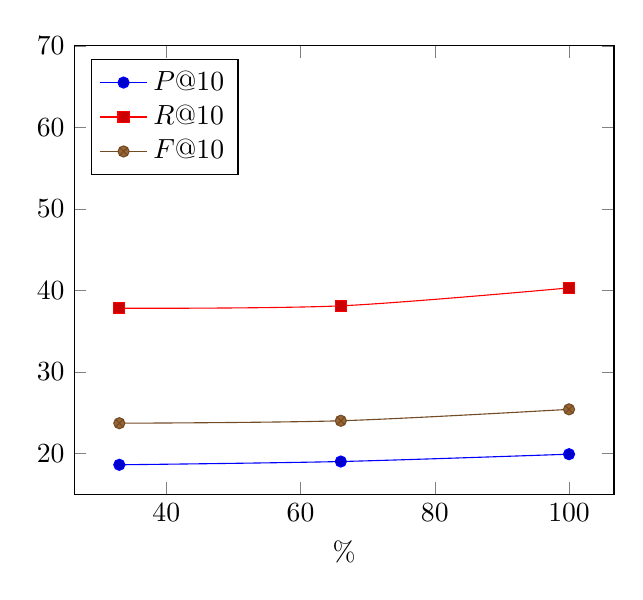
\begin{tikzpicture}%[font=\huge]
	\begin{axis}[smooth, xlabel={$\%$}, %ylabel={$\%$},
				 ymin=15, ymax=70, legend pos=north west]

		\addplot+ coordinates{(33, 18.6)(66, 19.0)(100, 19.9)};
		\addlegendentry{$P@10$}
		\addplot+ coordinates{(33, 37.8)(66, 38.1)(100, 40.3)};
		\addlegendentry{$R@10$}
		\addplot+ coordinates{(33, 23.7)(66, 24.0)(100, 25.4)};
		\addlegendentry{$F@10$}

		%\addplot+[mark=triangle*] coordinates{(33, 26.5)(66, 26.8)(100, 28.2)}; %\addlegendentry{P\@5}
		%\addplot+[mark=*] coordinates{(33, 27.9)(66, 27.8)(100, 29.6)}; %\addlegendentry{R\@5}
		%\addplot+[mark=square*] coordinates{(33, 26.0)(66, 26.0)(100, 27.6)}; %\addlegendentry{F\@5}
	\end{axis}
	\end{tikzpicture}
	}
	\caption{KP20k}
\end{subfigure}
%
\begin{subfigure}[t]{0.40\textwidth}
	\centering
	\resizebox{\linewidth}{!}{
	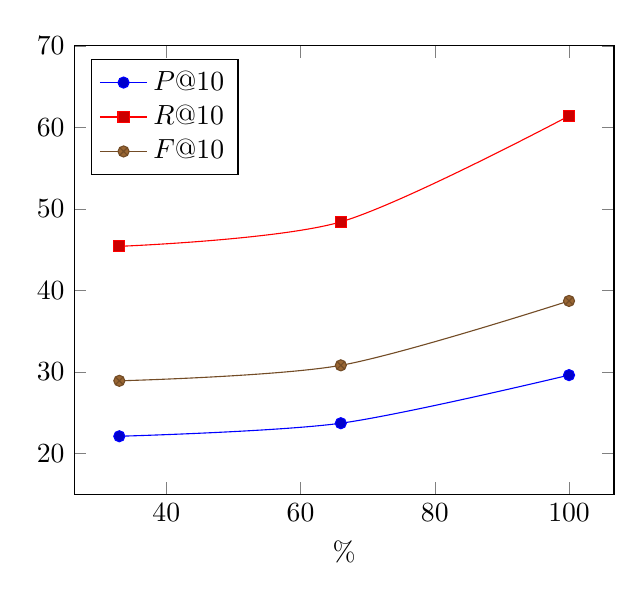
\begin{tikzpicture}%[font=\huge]
		\begin{axis}[
		    smooth,
		    xlabel={$\%$}, %ylabel={$\%$},
	    	ymin=15, ymax=70,
			legend pos=north west
		]

		\addlegendentry{$P@10$}
		\addplot coordinates{(33, 22.1)(66, 23.7)(100, 29.6)};
		
		\addlegendentry{$R@10$}
		\addplot coordinates{(33, 45.4)(66, 48.4)(100,61.4)};
		
		\addlegendentry{$F@10$}
		\addplot coordinates{(33, 28.9)(66, 30.8)(100, 38.7)};
		
		%\addplot+[smooth] coordinates{(33, 33.8)(100, 46.3)}; %\addlegendentry{P\@5}
		%\addplot+[smooth] coordinates{(33, 35.2)(100, 49.3)}; %\addlegendentry{R\@5}
		%\addplot+[smooth] coordinates{(33, 33.3)(100, 46.0)}; %\addlegendentry{F\@5}
		\end{axis}
	\end{tikzpicture}
	}
	\caption{KPTimes}
\end{subfigure}
    \vspace{-1em}
	\caption{Performances de CopyRNN en fonction de la taille du jeu de donnée d'entraînement.} \label{fig:train_percent}
\end{figure}
\fi

\begin{figure}
	\centering
	%\resizebox{.9\textwidth}{!}{
	\begin{tikzpicture}%[font=\huge]
	\begin{axis}[
	    scaled x ticks=false,
	    smooth, xlabel={$\#$ documents}, ylabel={$\%$ F@10},
		ymin=21, ymax=44,
		%legend pos=north east,
		legend pos=outer north east,
		xmin=0, xmax=600000,
		%xticklabels={0,100\,K,200\,K,300\,K,400\,K,500\,K},
        %xtick = {0,100000,200000,300000,400000,500000}]
        xticklabels={100\,K,300\,K,500\,K},
        xtick = {100000,300000,500000},
        ]

        \addplot+[color2,every mark/.append style={color=white,fill=color2},mark=*] coordinates{(86641, 34.4)(173282, 37.6)(259923, 38.7)};
        \addlegendentry{NYTimes}


        \addplot[color1,every mark/.append style={color=white,fill=color1},mark=X*] coordinates{(175696, 23.7)(351393, 24.0)(527090, 25.4)};
		\addlegendentry{KP20k}
	\end{axis}
	%https://tex.stackexchange.com/questions/413237/get-legend-outside-plot-on-tikz-and-customise-axis-labels
	%https://tex.stackexchange.com/questions/278530/how-i-can-customize-a-legend-on-pgfplots
	\iffalse
	\matrix [draw, matrix of nodes,
            anchor=south east,
        ] at (legend) {
        \multicolumn{2}{c}{Métrique} \\
        \ref{pgfplots:c2r1} & $P@10$ \\
        \ref{pgfplots:c2r2} & $R@10$ \\
        \ref{pgfplots:c2r3} & $F@10$ \\
        \multicolumn{2}{c}{Corpus} \\
        \ref{pgfplots:c2r2} & KP20k \\
        \ref{pgfplots:c2r2} & KPTimes \\
    };
	\fi
	%}
	\end{tikzpicture}
	\caption{Performances de CopyRNN (F@10) en fonction de la taille du jeu de données d'entraînement.}
	\label{fig:train_percent}
\end{figure}


Nous constatons que les performances des modèles s'améliorent progressivement à mesure que la taille de l'ensemble d'entraînement grandit.
%
L'ajout de données d'entraînement apporte des gains bien plus importants pour NYTimes ($+4,3$) tandis que les performances de CopyRNN peinent a augmenter ($+1,7$).
La courbe des modèles entraînés avec KP20k suggère que les données disponibles ne sont actuellement pas suffisantes pour atteindre un optimum en termes de performances, tandis que celle des modèles entraînés avec NYTimes semble converger vers un optimum.
%
En effet, l'annotation éditeur de NYTimes nécessite beaucoup moins d'exemple pour atteindre un optimum que l'annotation auteur de KP20k.
Ainsi, le manque de cohérence de l'annotation dans KP20k, que nous avons souligné dans les sections~\ref{sec:kptimes_valid} et \ref{sub:concepts_indexation_manuelle}, peut être la raison de ce résultat; l'apprentissage d'un modèle est intuitivement plus difficile avec des exemples étiquetés de manière peu cohérente. 
D'autres travaux étudient l'augmentation de la performance des méthodes en fonction de la quantité de données disponibles.
Par exemple, les travaux de \citet{ye_semi-supervised_2018} se placent dans un cadre où la quantité de données annotées est limitée (\num{40 000} documents). Ils montrent qu'enrichir l'ensemble d'entraînement avec des documents annotés automatiquement permet d'obtenir des performances comparables aux méthodes entraînées sur de plus grandes quantités de données annotées.
Nous pouvons aussi mentionner les travaux de \citet{martinc_tnt-kid_2021} qui tirent parti du transfert de connaissance d'un modèle de langue pré-entraîné.
Ils affinent ce modèle pour la tâche d'identification de mots-clés avec seulement \num{20 000} documents annotés. Cette méthode obtient des performances comparables avec les méthodes génératives de bout-en-bout entraînées avec de plus grandes quantités de données annotées.
%Notons que les deux travaux décrits se basent sur le jeu de données KP20k dont nous avons plusieurs fois exposé le manque de cohérence de l'annotation, les résultats auraient des 


\subsection{Choix du cadre expérimental pour l'évaluation}

La troisième question à laquelle nous voulons répondre dans cette étude est la suivante: \say{Quelles méthodes et quels jeux de données de référence devraient être inclus dans les travaux futurs pour mieux comprendre les avantages et les inconvénients des nouvelles méthodes proposées?}

%\definecolor{color3}{RGB}{208, 226, 194}
%\definecolor{cb}{RGB}{26, 40, 61}

\definecolor{ca}{RGB}{255, 0 , 0}
\definecolor{cb}{RGB}{255, 255, 255}

% https://tex.stackexchange.com/questions/401370/how-to-interpolate-two-colors-in-a-cell
% \newcommand\Heat[1]{% \Heat{number in the interval [-1,1]}
%    \pgfmathparse{int(50+50*#1)}% map number in [-1,1] to [0,100]
%    \edef\HeatCell{\noexpand\cellcolor{red!\pgfmathresult!blue}}%
%    \HeatCell$#1$%
%}


\begin{figure}
\centering
\begin{subfigure}{0.49\textwidth}
    \centering
\resizebox{0.9\linewidth}{!}{
\begin{tikzpicture}[square/.append style={inner sep=2.3}]

    \foreach \x [count=\n] in {
        TextRank,EmbedRank,PositionRank,FirstPhrases,MPRank,Kea,\tfidf{},CopyRNN,CorrRNN
    } {
        \node[rotate=-45,xshift=0.6cm,anchor=east] at (\n-1,1) {\x};
        \node[xshift=0.5cm,anchor=east] at (-1,-\n+1) {\x};
    }
        \node at (0,-1) [square,fill=color3!68!cb] {6,8};
        \node at (0,-2) [square,fill=color3!70!cb] {7,0};
        \node at (0,-3) [square,fill=color3!40!cb] {4,0};
        \node at (0,-4) [square,fill=color3!40!cb] {4,0};
        \node at (0,-5) [square,fill=color3!50!cb] {5,0};
        \node at (0,-6) [square,fill=color3!60!cb] {6,0};
        \node at (0,-7) [square,fill=color3!22!cb] {2,2};
        \node at (0,-8) [square,fill=color3!24!cb] {2,4};

        \node at (1,0) [square,fill=color3!68!cb] {6,8};
        \node at (1,-2) [square,fill=color3!69!cb] {6,9};
        \node at (1,-3) [square,fill=color3!45!cb] {4,5};
        \node at (1,-4) [square,fill=color3!46!cb] {4,6};
        \node at (1,-5) [square,fill=color3!53!cb] {5,3};
        \node at (1,-6) [square,fill=color3!56!cb] {5,6};
        \node at (1,-7) [square,fill=color3!27!cb] {2,7};
        \node at (1,-8) [square,fill=color3!27!cb] {2,7};

        \node at (2,0) [square,fill=color3!70!cb] {7,0};
        \node at (2,-1) [square,fill=color3!69!cb] {6,9};
        \node at (2,-3) [square,fill=color3!55!cb] {5,5};
        \node at (2,-4) [square,fill=color3!52!cb] {5,2};
        \node at (2,-5) [square,fill=color3!62!cb] {6,2};
        \node at (2,-6) [square,fill=color3!61!cb] {6,1};
        \node at (2,-7) [square,fill=color3!29!cb] {2,9};
        \node at (2,-8) [square,fill=color3!30!cb] {3,0};

        \node at (3,0) [square,fill=color3!40!cb] {4,0};
        \node at (3,-1) [square,fill=color3!45!cb] {4,5};
        \node at (3,-2) [square,fill=color3!55!cb] {5,5};
        \node at (3,-4) [square,fill=color3!70!cb] {7,0};
        \node at (3,-5) [square,fill=color3!75!cb] {7,5};
        \node at (3,-6) [square,fill=color3!52!cb] {5,2};
        \node at (3,-7) [square,fill=color3!28!cb] {2,8};
        \node at (3,-8) [square,fill=color3!28!cb] {2,8};

        \node at (4,0) [square,fill=color3!40!cb] {4,0};
        \node at (4,-1) [square,fill=color3!46!cb] {4,6};
        \node at (4,-2) [square,fill=color3!52!cb] {5,2};
        \node at (4,-3) [square,fill=color3!70!cb] {7,0};
        \node at (4,-5) [square,fill=color3!67!cb] {6,7};
        \node at (4,-6) [square,fill=color3!54!cb] {5,4};
        \node at (4,-7) [square,fill=color3!29!cb] {2,9};
        \node at (4,-8) [square,fill=color3!28!cb] {2,8};

        \node at (5,0) [square,fill=color3!50!cb] {5,0};
        \node at (5,-1) [square,fill=color3!53!cb] {5,3};
        \node at (5,-2) [square,fill=color3!62!cb] {6,2};
        \node at (5,-3) [square,fill=color3!75!cb] {7,5};
        \node at (5,-4) [square,fill=color3!67!cb] {6,7};
        \node at (5,-6) [square,fill=color3!72!cb] {7,2};
        \node at (5,-7) [square,fill=color3!30!cb] {3,0};
        \node at (5,-8) [square,fill=color3!30!cb] {3,0};

        \node at (6,0) [square,fill=color3!60!cb] {6,0};
        \node at (6,-1) [square,fill=color3!56!cb] {5,6};
        \node at (6,-2) [square,fill=color3!61!cb] {6,1};
        \node at (6,-3) [square,fill=color3!52!cb] {5,2};
        \node at (6,-4) [square,fill=color3!54!cb] {5,4};
        \node at (6,-5) [square,fill=color3!72!cb] {7,2};
        \node at (6,-7) [square,fill=color3!26!cb] {2,6};
        \node at (6,-8) [square,fill=color3!27!cb] {2,7};

        \node at (7,0) [square,fill=color3!22!cb] {2,2};
        \node at (7,-1) [square,fill=color3!27!cb] {2,7};
        \node at (7,-2) [square,fill=color3!29!cb] {2,9};
        \node at (7,-3) [square,fill=color3!28!cb] {2,8};
        \node at (7,-4) [square,fill=color3!29!cb] {2,9};
        \node at (7,-5) [square,fill=color3!30!cb] {3,0};
        \node at (7,-6) [square,fill=color3!26!cb] {2,6};
        \node at (7,-8) [square,fill=color3!51!cb] {5,1};

        \node at (8,0) [square,fill=color3!24!cb] {2,4};
        \node at (8,-1) [square,fill=color3!27!cb] {2,7};
        \node at (8,-2) [square,fill=color3!30!cb] {3,0};
        \node at (8,-3) [square,fill=color3!28!cb] {2,8};
        \node at (8,-4) [square,fill=color3!28!cb] {2,8};
        \node at (8,-5) [square,fill=color3!30!cb] {3,0};
        \node at (8,-6) [square,fill=color3!27!cb] {2,7};
        \node at (8,-7) [square,fill=color3!51!cb] {5,1};

\end{tikzpicture}
}
\caption{Notices scientifiques.}
\end{subfigure}
%
\begin{subfigure}{0.49\textwidth}
\centering
\resizebox{0.9\linewidth}{!}{
\begin{tikzpicture}[square/.append style={inner sep=2.3}]

    \foreach \x [count=\n] in {
        TextRank,EmbedRank,PositionRank,FirstPhrases,MPRank,Kea,\tfidf{},CopyRNN,CorrRNN
    } {
        \node[rotate=-45,xshift=0.6cm,anchor=east] at (\n-1,1) {\x};
        \node[xshift=0.5cm,anchor=east] at (-1,-\n+1) {\x};
    }
        \node at (0,-1) [square,fill=color3!25!cb] {2,5};
        \node at (0,-2) [square,fill=color3!53!cb] {5,3};
        \node at (0,-3) [square,fill=color3!5!cb] {0,5};
        \node at (0,-4) [square,fill=color3!5!cb] {0,5};
        \node at (0,-5) [square,fill=color3!4!cb] {0,4};
        \node at (0,-6) [square,fill=color3!3!cb] {0,3};
        \node at (0,-7) [square,fill=color3!3!cb] {0,3};
        \node at (0,-8) [square,fill=color3!4!cb] {0,4};

        \node at (1,0) [square,fill=color3!25!cb] {2,5};
        \node at (1,-2) [square,fill=color3!24!cb] {2,4};
        \node at (1,-3) [square,fill=color3!4!cb] {0,4};
        \node at (1,-4) [square,fill=color3!5!cb] {0,5};
        \node at (1,-5) [square,fill=color3!5!cb] {0,5};
        \node at (1,-6) [square,fill=color3!5!cb] {0,5};
        \node at (1,-7) [square,fill=color3!4!cb] {0,4};
        \node at (1,-8) [square,fill=color3!4!cb] {0,4};

        \node at (2,0) [square,fill=color3!53!cb] {5,3};
        \node at (2,-1) [square,fill=color3!24!cb] {2,4};
        \node at (2,-3) [square,fill=color3!12!cb] {1,2};
        \node at (2,-4) [square,fill=color3!10!cb] {1,0};
        \node at (2,-5) [square,fill=color3!9!cb] {0,9};
        \node at (2,-6) [square,fill=color3!9!cb] {0,9};
        \node at (2,-7) [square,fill=color3!7!cb] {0,7};
        \node at (2,-8) [square,fill=color3!9!cb] {0,9};

        \node at (3,0) [square,fill=color3!5!cb] {0,5};
        \node at (3,-1) [square,fill=color3!4!cb] {0,4};
        \node at (3,-2) [square,fill=color3!12!cb] {1,2};
        \node at (3,-4) [square,fill=color3!36!cb] {3,6};
        \node at (3,-5) [square,fill=color3!20!cb] {2,0};
        \node at (3,-6) [square,fill=color3!16!cb] {1,6};
        \node at (3,-7) [square,fill=color3!17!cb] {1,7};
        \node at (3,-8) [square,fill=color3!23!cb] {2,3};

        \node at (4,0) [square,fill=color3!5!cb] {0,5};
        \node at (4,-1) [square,fill=color3!5!cb] {0,5};
        \node at (4,-2) [square,fill=color3!10!cb] {1,0};
        \node at (4,-3) [square,fill=color3!36!cb] {3,6};
        \node at (4,-5) [square,fill=color3!41!cb] {4,1};
        \node at (4,-6) [square,fill=color3!36!cb] {3,6};
        \node at (4,-7) [square,fill=color3!22!cb] {2,2};
        \node at (4,-8) [square,fill=color3!20!cb] {2,0};

        \node at (5,0) [square,fill=color3!4!cb] {0,4};
        \node at (5,-1) [square,fill=color3!5!cb] {0,5};
        \node at (5,-2) [square,fill=color3!9!cb] {0,9};
        \node at (5,-3) [square,fill=color3!20!cb] {2,0};
        \node at (5,-4) [square,fill=color3!41!cb] {4,1};
        \node at (5,-6) [square,fill=color3!85!cb] {8,5};
        \node at (5,-7) [square,fill=color3!29!cb] {2,9};
        \node at (5,-8) [square,fill=color3!20!cb] {2,0};

        \node at (6,0) [square,fill=color3!3!cb] {0,3};
        \node at (6,-1) [square,fill=color3!5!cb] {0,5};
        \node at (6,-2) [square,fill=color3!9!cb] {0,9};
        \node at (6,-3) [square,fill=color3!16!cb] {1,6};
        \node at (6,-4) [square,fill=color3!36!cb] {3,6};
        \node at (6,-5) [square,fill=color3!85!cb] {8,5};
        \node at (6,-7) [square,fill=color3!27!cb] {2,7};
        \node at (6,-8) [square,fill=color3!18!cb] {1,8};

        \node at (7,0) [square,fill=color3!3!cb] {0,3};
        \node at (7,-1) [square,fill=color3!4!cb] {0,4};
        \node at (7,-2) [square,fill=color3!7!cb] {0,7};
        \node at (7,-3) [square,fill=color3!17!cb] {1,7};
        \node at (7,-4) [square,fill=color3!22!cb] {2,2};
        \node at (7,-5) [square,fill=color3!29!cb] {2,9};
        \node at (7,-6) [square,fill=color3!27!cb] {2,7};
        \node at (7,-8) [square,fill=color3!37!cb] {3,7};

        \node at (8,0) [square,fill=color3!4!cb] {0,4};
        \node at (8,-1) [square,fill=color3!4!cb] {0,4};
        \node at (8,-2) [square,fill=color3!9!cb] {0,9};
        \node at (8,-3) [square,fill=color3!23!cb] {2,3};
        \node at (8,-4) [square,fill=color3!20!cb] {2,0};
        \node at (8,-5) [square,fill=color3!20!cb] {2,0};
        \node at (8,-6) [square,fill=color3!18!cb] {1,8};
        \node at (8,-7) [square,fill=color3!37!cb] {3,7};

\end{tikzpicture}
}
\caption{Articles scientifiques.}
\end{subfigure}
%
\begin{subfigure}{0.49\textwidth}
    \centering
\resizebox{0.9\linewidth}{!}{
\begin{tikzpicture}[square/.append style={inner sep=2.3}]

    \foreach \x [count=\n] in {
        TextRank,EmbedRank,PositionRank,FirstPhrases,MPRank,Kea,\tfidf{},CopyRNN,CorrRNN
    } {
        \node[rotate=-45,xshift=0.6cm,anchor=east] at (\n-1,1) {\x};
        \node[xshift=0.5cm,anchor=east] at (-1,-\n+1) {\x};
    }
        \node at (0,-1) [square,fill=color3!42!cb] {4,2};
        \node at (0,-2) [square,fill=color3!54!cb] {5,4};
        \node at (0,-3) [square,fill=color3!17!cb] {1,7};
        \node at (0,-4) [square,fill=color3!19!cb] {1,9};
        \node at (0,-5) [square,fill=color3!22!cb] {2,2};
        \node at (0,-6) [square,fill=color3!23!cb] {2,3};
        \node at (0,-7) [square,fill=color3!5!cb] {0,5};
        \node at (0,-8) [square,fill=color3!5!cb] {0,5};

        \node at (1,0) [square,fill=color3!42!cb] {4,2};
        \node at (1,-2) [square,fill=color3!41!cb] {4,1};
        \node at (1,-3) [square,fill=color3!19!cb] {1,9};
        \node at (1,-4) [square,fill=color3!25!cb] {2,5};
        \node at (1,-5) [square,fill=color3!26!cb] {2,6};
        \node at (1,-6) [square,fill=color3!26!cb] {2,6};
        \node at (1,-7) [square,fill=color3!7!cb] {0,7};
        \node at (1,-8) [square,fill=color3!6!cb] {0,6};

        \node at (2,0) [square,fill=color3!54!cb] {5,4};
        \node at (2,-1) [square,fill=color3!41!cb] {4,1};
        \node at (2,-3) [square,fill=color3!38!cb] {3,8};
        \node at (2,-4) [square,fill=color3!35!cb] {3,5};
        \node at (2,-5) [square,fill=color3!39!cb] {3,9};
        \node at (2,-6) [square,fill=color3!34!cb] {3,4};
        \node at (2,-7) [square,fill=color3!11!cb] {1,1};
        \node at (2,-8) [square,fill=color3!13!cb] {1,3};

        \node at (3,0) [square,fill=color3!17!cb] {1,7};
        \node at (3,-1) [square,fill=color3!19!cb] {1,9};
        \node at (3,-2) [square,fill=color3!38!cb] {3,8};
        \node at (3,-4) [square,fill=color3!50!cb] {5,0};
        \node at (3,-5) [square,fill=color3!50!cb] {5,0};
        \node at (3,-6) [square,fill=color3!33!cb] {3,3};
        \node at (3,-7) [square,fill=color3!14!cb] {1,4};
        \node at (3,-8) [square,fill=color3!15!cb] {1,5};

        \node at (4,0) [square,fill=color3!19!cb] {1,9};
        \node at (4,-1) [square,fill=color3!25!cb] {2,5};
        \node at (4,-2) [square,fill=color3!35!cb] {3,5};
        \node at (4,-3) [square,fill=color3!50!cb] {5,0};
        \node at (4,-5) [square,fill=color3!55!cb] {5,5};
        \node at (4,-6) [square,fill=color3!47!cb] {4,7};
        \node at (4,-7) [square,fill=color3!17!cb] {1,7};
        \node at (4,-8) [square,fill=color3!16!cb] {1,6};

        \node at (5,0) [square,fill=color3!22!cb] {2,2};
        \node at (5,-1) [square,fill=color3!26!cb] {2,6};
        \node at (5,-2) [square,fill=color3!39!cb] {3,9};
        \node at (5,-3) [square,fill=color3!50!cb] {5,0};
        \node at (5,-4) [square,fill=color3!55!cb] {5,5};
        \node at (5,-6) [square,fill=color3!76!cb] {7,6};
        \node at (5,-7) [square,fill=color3!18!cb] {1,8};
        \node at (5,-8) [square,fill=color3!17!cb] {1,7};

        \node at (6,0) [square,fill=color3!23!cb] {2,3};
        \node at (6,-1) [square,fill=color3!26!cb] {2,6};
        \node at (6,-2) [square,fill=color3!34!cb] {3,4};
        \node at (6,-3) [square,fill=color3!33!cb] {3,3};
        \node at (6,-4) [square,fill=color3!47!cb] {4,7};
        \node at (6,-5) [square,fill=color3!76!cb] {7,6};
        \node at (6,-7) [square,fill=color3!17!cb] {1,7};
        \node at (6,-8) [square,fill=color3!16!cb] {1,6};

        \node at (7,0) [square,fill=color3!5!cb] {0,5};
        \node at (7,-1) [square,fill=color3!7!cb] {0,7};
        \node at (7,-2) [square,fill=color3!11!cb] {1,1};
        \node at (7,-3) [square,fill=color3!14!cb] {1,4};
        \node at (7,-4) [square,fill=color3!17!cb] {1,7};
        \node at (7,-5) [square,fill=color3!18!cb] {1,8};
        \node at (7,-6) [square,fill=color3!17!cb] {1,7};
        \node at (7,-8) [square,fill=color3!26!cb] {2,6};

        \node at (8,0) [square,fill=color3!5!cb] {0,5};
        \node at (8,-1) [square,fill=color3!6!cb] {0,6};
        \node at (8,-2) [square,fill=color3!13!cb] {1,3};
        \node at (8,-3) [square,fill=color3!15!cb] {1,5};
        \node at (8,-4) [square,fill=color3!16!cb] {1,6};
        \node at (8,-5) [square,fill=color3!17!cb] {1,7};
        \node at (8,-6) [square,fill=color3!16!cb] {1,6};
        \node at (8,-7) [square,fill=color3!26!cb] {2,6};

\end{tikzpicture}
}
\caption{Articles journalistiques.}
\end{subfigure}

\caption{Nombre moyen de mots-clés en commun dans les 10 premiers mots-clés de chacune des méthodes.}
\label{fig:intersect}

\end{figure}


Il est important de disposer de méthodes de base dont les performances sont proches de l'état de l'art pour pouvoir s'y comparer.
Les résultats de notre évaluation nous permettent de donner des indications quant au choix des méthodes les plus pertinentes à utiliser comme méthodes de base.
Tout d'abord, les méthodes neuronales, lorsqu'elles sont correctement entraînées, surpassent nettement toutes les autres méthodes et représentent l'état de l'art.
Ainsi et parce qu'elle obtient les meilleurs résultats, la méthode CopyRNN devrait être incluse dans les travaux futurs à des fins de comparaison.
Toutefois, dans un cadre non supervisé ou dans un scénario où les données sont rares, et donc où les modèles neuronaux ne peuvent être utilisés, la situation est moins claire.

Par ailleurs, les méthodes FirstPhrases, \tfidf{}, MPRank et Kea qui obtiennent des scores similaires devraient aussi être utilisés à titre de comparaison.
Par contre, la méthode TextRank, bien qu'elle soit une méthode pionnière, n'est pas une bonne méthode de base car ses performances sont bien trop basses par rapport à l'état de l'art.

Pour éclaircir le choix des méthodes en chaîne de traitement qui devraient être incluses dans les futurs travaux, nous avons mené une série d'expériences visant à comparer les sorties des méthodes deux à deux.
La motivation derrière ces expériences réside dans le fait qu'inclure plusieurs méthodes qui se comportent de manière similaire est d'un intérêt limité.
Les similarités entre les sorties des méthodes, en termes de nombre de mots-clés en commun, sont représentées sous forme de \foreign{heatmap} dans la figure~\ref{fig:intersect}.
Globalement, nous observons des tendances différentes pour chaque genre de documents.
Plus le document est court, plus les sorties sont similaires, ce qui est principalement dû à un plus petit nombre de mots-clé candidats.
Nous apercevons aussi trois clusters de méthodes dont les mots-clés produits sont similaires: TextRank, EmbedRank et PositionRank; FirstPhrases, MPRank, Kea et \tfidf{}; et enfin les méthodes génératives CopyRNN et CorrRNN.
En particulier, \tfidf{} et Kea produisent des mots-clés toujours assez similaires, ce qui s'explique par l'utilisation du score de \tfidf{} par Kea pour classifier les mots-clés.
Notons aussi que les trois meilleures méthodes non supervisées, à savoir FirstPhrases, \tfidf{} et MPRank, génèrent des mots-clés très similaires.
Compte tenu de cela, et de leurs performances rapportées dans le tableau~\ref{tab:results}, nous soutenons que \tfidf{} (ou Kea si des données d'entraînement sont disponibles) et FirstPhrases devraient être considérées comme des méthodes de base non supervisées dans les travaux futurs. Elles produisent, en effet, des mots-clés différents et sont parmi les méthodes les plus performantes.

Ces recommandations de méthodes de base ont également une incidence sur le choix des jeux de données de référence à utiliser.
%
Les modèles neuronaux étant gourmands en données, KP20k et KPTimes sont les options par défaut pour les notices scientifiques et les articles journalistiques.
%
Pour les articles scientifiques, nous recommandons d'utiliser SemEval pour deux raisons: 1) il est largement utilisé par les études existantes; et 2) il fournit une référence doublement annotée (annotation auteur et lecteur) qui atténue dans une certaine mesure les incohérences d'annotation.
%Le jeu de données Inspec, même s'il est annoté par des indexeurs professionnels permet peu de différencier

\section{Conclusion}

% chapeau
Dans ce chapitre, nous avons présenté une évaluation à grande échelle de méthodes de production automatique de mots-clés réalisée sur plusieurs jeux de données contenant des documents de genres différents.
%
Notre objectif était de répondre à trois questions concernant les progrès réalisés par les méthodes, l'importance de la qualité de l'annotation et les méthodes et jeux de données à utiliser pour les travaux futurs. Pour atteindre cet objectif, nous avons mis en place un cadre expérimental partagé, disponible sur un dépôt public\footnote{\url{https://github.com/ygorg/JCDL_2020_KPE_Eval}} afin de faciliter la reproductibilité des expériences ainsi que la réutilisation du cadre expérimental.

% 5.2.1 résumé des résultats
Nos résultats montrent que les méthodes neuronales génératives sont globalement meilleures mais que les méthodes de base (comme \tfidf{}) restent compétitives.
%Ces résultats nous ont permis d'émettre des recommandations sur les méthodes et les jeux de données à inclure dans les travaux futurs. 
% 5.2.2 impact des références
Nous avons aussi étudié l'impact des types de mots-clés de référence sur l'évaluation automatique.
Ainsi, nous avons trouvé que l'évaluation sur les mots-clés auteurs sous-estime les performances des méthodes évaluées par rapport à une évaluation sur les mots-clés indexeurs, plus qualitatifs.
Ces annotations indexeurs sont coûteuses en temps et en argent comme nous l'avons vu dans la section~\ref{sub:concepts_indexation_manuelle}.
C'est pourquoi, plutôt que de construire de nouvelles collections de test annotées en mots-clés indexeurs, nous préconisons le développement de nouveaux processus d'évaluation automatique.

% 5.2.3 courbe d'apprentissage -> KPTimes ?
Nous avons montré que les méthodes génératives neuronales, qui sont les plus performantes des méthodes évaluées ici, nécessitent de grandes quantités de données pour être entraînées.
Pour savoir si les données actuellement disponibles sont suffisantes à leur entraînement, nous avons évalué ces méthodes après les avoir entraînées avec différentes quantités de données.
Notre expérience montre que les performances des modèles augmentent avec l'ajout de données d'entraînement mais que cette augmentation est bien plus élevée avec KPTimes qu'avec KP20k.
Nous en concluons que la faible cohérence de l'annotation auteur complexifie l'entraînement (comme nous l'avons vu dans la section~\ref{sub:kptimes_generalisation}) et limite la modélisation de cette annotation par le modèle.

% 5.2.4 choix des cadre expérimentaux futurs
Notre but avec cette étude était de recommander les méthodes à utiliser à minima pour valider les nouvelles contributions. Nous recommandons donc \tfidf{} (ou Kea si des données d'apprentissage sont disponibles) et FirstPhrases comme méthodes de base ainsi que CopyRNN.
Les deux premières sont non supervisées et peu gourmandes en termes de ressources, elles peuvent donc être appliquées à tout jeux de données.
La dernière, CopyRNN, obtient aujourd'hui des performances état de l'art et permet de produire des mots-clés absents mais nécessite une grande puissance de calcul et est peu généralisable à de nouveaux domaines.
%Elles sont ainsi bien plus gourmandes en ressource que les méthodes non supervisées. Du fait de leurs faibles capacités de généralisation, elles sont aussi très dépendantes du domaine des documents grâce auxquels elles ont été entraînées.
Pour les jeux de données, nous recommandons l'utilisation de KP20k et KPTimes de par leur taille ainsi que SemEval-2010 qui contient une double annotation auteur et lecteur. Ces trois jeux de données permettent de couvrir l'ensemble des genres de documents couramment utilisés: les notices scientifiques, les articles scientifiques et les articles journalistiques.

Finalement, nos expériences ont mis en évidence plusieurs problèmes lors de l'évaluation des méthodes de production de mots-clés, notamment le choix des jeux de données à utiliser, ainsi que la qualité de leurs annotations.
Dès lors, une autre façon d'évaluer l'efficacité de ces méthodes serait d'explorer leur impact dans des cadres applicatifs.
Dans le chapitre suivant nous nous intéresserons à l'évaluation de la production automatique de mots-clés dans le cadre de la recherche d'information.